\documentclass[11pt,a4paper]{article}
\usepackage[T1]{fontenc}
\usepackage[utf8]{inputenc}
\usepackage{lmodern}
\usepackage{amsmath,amssymb,amsthm,mathtools,mathrsfs}
\usepackage{graphicx,float,xcolor,multicol}
\usepackage[shortlabels]{enumitem}
\usepackage[margin=27mm]{geometry}
\usepackage{microtype,needspace,placeins}
\usepackage{tikz,tikz-cd}
\usetikzlibrary{arrows.meta,calc,positioning,patterns,decorations.pathreplacing}
\usepackage[colorlinks=true,linkcolor=teal,urlcolor=teal,citecolor=teal]{hyperref}
\setlength{\parindent}{0pt}
\setlength{\parskip}{.6em}
\setcounter{secnumdepth}{0}
\allowdisplaybreaks
\raggedbottom
\providecommand{\cross}{\times}
\DeclareUnicodeCharacter{2020}{\ensuremath{\dagger}}
\DeclareMathOperator{\supp}{supp}
\DeclareMathOperator*{\esssup}{ess\,sup}
\providecommand{\chapter}{\section}
\newenvironment{tool}[2]{\subsection*{Tool #1 --- #2}}{}
\newcommand{\ToolRef}[1]{Tool #1}
\newcommand{\FigureTag}[2]{\textit{Figure #1}}
\newcommand{\Result}[1]{\subsection*{#1}}
\newcommand{\Application}[1]{\subsubsection*{Application\if\relax\detokenize{#1}\relax\else\space--- #1\fi}}
\newcommand{\ProofHeading}{\par\textit{Proof.}\space}
\newcommand{\ProofOf}[1]{\par\textit{Proof of #1.}\space}
\newcommand{\RemarkHeading}{\par\textbf{Remark.}\space}
\newcommand{\NoteHeading}{\par\textbf{Note.}\space}
\newcommand{\ExerciseHeading}{\par\textbf{Exercise.}\space}

% Rendering support only; mathematical text is in each independent post.
\usepackage{booktabs,array,longtable}
\definecolor{HandoutBlue}{HTML}{2F6690}
\definecolor{HandoutNavy}{HTML}{17365D}
\newtheorem{theorem}{Theorem}
\newtheorem{lemma}[theorem]{Lemma}
\newtheorem{proposition}[theorem]{Proposition}
\newtheorem{corollary}[theorem]{Corollary}
\newtheorem{conjecture}[theorem]{Conjecture}
\newtheorem{definition}{Definition}
\newtheorem{example}{Example}
\newtheorem{namedtoolcounter}{Tool}
\newenvironment{namedtool}[1]{\begin{namedtoolcounter}[#1]}{\end{namedtoolcounter}}
\newtheorem*{claim}{Claim}
\newtheorem*{remark}{Remark}
\newtheorem*{exercise}{Exercise}
\newtheorem*{question}{Question}
\newtheorem*{observation}{Observation}
\newcommand{\SourceChapter}[2]{\section*{#2}}
\newcommand{\Lecture}[2]{\section*{Lecture #1: #2}}
\newcommand{\unclear}[1]{\textit{[unclear: #1]}}
\newcommand{\sourcegap}{\textit{[unfinished in the source]}}
\DeclareMathOperator{\dist}{dist}
\DeclareMathOperator{\id}{id}
\DeclareMathOperator{\Hol}{Hol}
\DeclareMathOperator{\Per}{Per}
\DeclareMathOperator{\Fix}{Fix}
\DeclareMathOperator{\diam}{diam}
\DeclareMathOperator{\Var}{Var}
\DeclareMathOperator{\Leb}{Leb}
\DeclareMathOperator{\Hom}{Hom}
\DeclareMathOperator{\End}{End}
\DeclareMathOperator{\Ann}{Ann}
\DeclareMathOperator{\Spec}{Spec}
\DeclareMathOperator{\Max}{Max}
\DeclareMathOperator{\Ob}{Ob}
\DeclareMathOperator{\Tor}{Tor}
\DeclareMathOperator{\Ass}{Ass}
\DeclareMathOperator{\Mor}{Mor}
\DeclareMathOperator{\Fun}{Fun}
\DeclareMathOperator{\Nat}{Nat}
\DeclareMathOperator{\Cone}{Cone}
\DeclareMathOperator{\MCG}{MCG}
\DeclareMathOperator{\Aut}{Aut}
\DeclareMathOperator{\Deck}{Deck}
\DeclareMathOperator{\SL}{SL}
\DeclareMathOperator{\PSL}{PSL}
\DeclareMathOperator{\Area}{Area}
\DeclareMathOperator{\im}{im}
\DeclareMathOperator{\PSh}{PSh}
\newcommand{\CRing}{\mathsf{CRings}}
\newcommand{\AMod}{A\text{-}\mathsf{Mod}}
\newcommand{\Ab}{\mathsf{Ab}}
\newcommand{\Z}{\mathbb Z}
\newcommand{\Q}{\mathbb Q}
\newcommand{\R}{\mathbb R}
\newcommand{\C}{\mathbb C}
\newcommand{\N}{\mathbb N}
\newcommand{\kk}{\mathbb k}
\renewcommand{\aa}{\mathfrak a}
\newcommand{\bb}{\mathfrak b}
\newcommand{\pp}{\mathfrak p}
\newcommand{\qq}{\mathfrak q}
\newcommand{\mm}{\mathfrak m}
\newcommand{\nn}{\mathfrak n}
\newcommand{\rad}{\mathrm r}
\newcommand{\cat}[1]{\mathsf{#1}}
\setcounter{secnumdepth}{0}
\allowdisplaybreaks

\graphicspath{{figures/miscellaneous/}}
\begin{document}
\section*{Orientation and Covering Maps}
% BLOG-CONTENT-BEGIN
\begin{center}\small S. Viswanathan\end{center}
% Source page 1
% Source page 2
In this exposition we shall see some covering-space-theoretic implications
of orientability. We have seen covering space theory in calculating
fundamental groups, lifting holomorphic branches, studying covering spaces,
classifying manifolds, and pushing certain invariant metrics.
We shall now see yet another application: the Orientation Covering Theorem.

Given a covering map $\pi\colon E\to M$, there are fundamentally three
objects associated to it: $\pi_1(M)$, the fundamental group;
$\Aut_\pi(E)$, the group of deck transformations; and $E$, the covering space.
Let us see what these objects have to say about the orientability of $M$.
\setcounter{theorem}{13}\begin{theorem}
\label{thm:m4-deck-orientation}
Let $\pi\colon E\to M$ be a smooth normal covering map, where $E$ is a
connected, oriented smooth manifold and $M$ is a smooth manifold.
Then $M$ is orientable if and only if the action of $\Aut_\pi(E)$ on $E$
is orientation-preserving.
\end{theorem}
From the action of $\Aut_\pi(E)$, a Lie group in its own right, one can
determine the orientability of $M$. But one can do better by considering
a particular covering space. Before we do that, here is an example.
% Source page 4
\setcounter{example}{5}\begin{example}
The map $q\colon S^n\to\mathbb{RP}^n$ is a covering map.
For $n>1$, $S^n$ is simply connected, and
$\pi_1(\mathbb{RP}^n)=\mathbb Z/2\mathbb Z\cong\Aut_q(S^n)$.
The nontrivial element of $\Aut_q(S^n)$ is $\alpha(x)=-x$, the antipodal map.
The map $\alpha$ is orientation-preserving if and only if $2\nmid n$.
Therefore $\mathbb{RP}^n$ is orientable if and only if $2\nmid n$.
Also, $\mathbb{RP}^1$ is orientable.
\end{example}
\subsection{Orientation Covering}
We are now going to construct a particular covering map for $M$ to help
us analyse its orientability. Define
\[
 \widehat M:=\{(p,O_p):p\in M,\ O_p\text{ is an orientation of }T_pM\},
 \qquad
 \widehat\pi\colon\widehat M\to M,\quad\widehat\pi(p,O_p):=p.
\]
This is called the \emph{orientation covering} of $M$.
\setcounter{theorem}{14}\begin{proposition}
\label{prop:m4-smooth-cover}
Given the orientation covering $\widehat\pi\colon\widehat M\to M$, one can
give $\widehat M$ a smooth structure such that:
\begin{enumerate}[label=(\alph*)]
 \setcounter{enumi}{0}\item $\widehat\pi\colon\widehat M\to M$ is a smooth covering map.
 % Source page 5
 \setcounter{enumi}{1}\item A connected open set $U\subset M$ is evenly covered by
 $\widehat\pi$ if and only if $U$ is orientable.
\end{enumerate}
\end{proposition}
% Source page 7
\setcounter{theorem}{15}\begin{theorem}[Orientation Covering Theorem]
Let $M$ be a connected smooth manifold and
$\widehat\pi\colon\widehat M\to M$ its orientation covering.
If $M$ is orientable, then $\widehat M$ has two components.
If $M$ is not orientable, then $\widehat M$ is connected.
\end{theorem}
\begin{proof}
If $M$ is orientable, then, being connected and open, it is evenly covered
by Proposition~\href{https://codezen1729.github.io/math-blog/\#/post/orientation-and-covering-maps}{15}. Since
$|\widehat\pi^{-1}(\{p\})|=2$, we have
\[
 \widehat\pi^{-1}(M)=M^+\sqcup M^-=\widehat M,\qquad
 \widehat\pi|_{M^\pm}\colon M^\pm\cong M.
\]
If $M$ is not orientable, let $W$ be a component of $\widehat M$.
The restriction $\widehat\pi|_W$ is a covering map. Since $W$ is connected,
the degree of $\widehat\pi|_W$ is invariant on $W$, so its fibres have
cardinality either $1$ or $2$.
If their cardinality were $1$, then $\widehat\pi|_W\colon W\to M$ would
be a diffeomorphism, making $M$ orientable.
Therefore their cardinality is $2$, and surjectivity of
$\widehat\pi|_W$ implies $W=\widehat M$, which is connected.
% Typo corrected: the source says a component of M where the entire argument requires a component of M-hat.
\end{proof}
In hindsight, $\widehat M$ may seem tailor-made to capture orientability
by merely restating it in a different form on a made-up space $\widehat M$.
But that is not the
% Source page 8
case. The right way to think about it intuitively is via an ambient
manifold. Consider surfaces in $\mathbb R^3$, say a page.
The space $\widehat M$ is basically what you get after slicing the surface
along its extra dimension, which in $\mathbb R^3$ would be its thickness.
\begin{figure}[H]
 \centering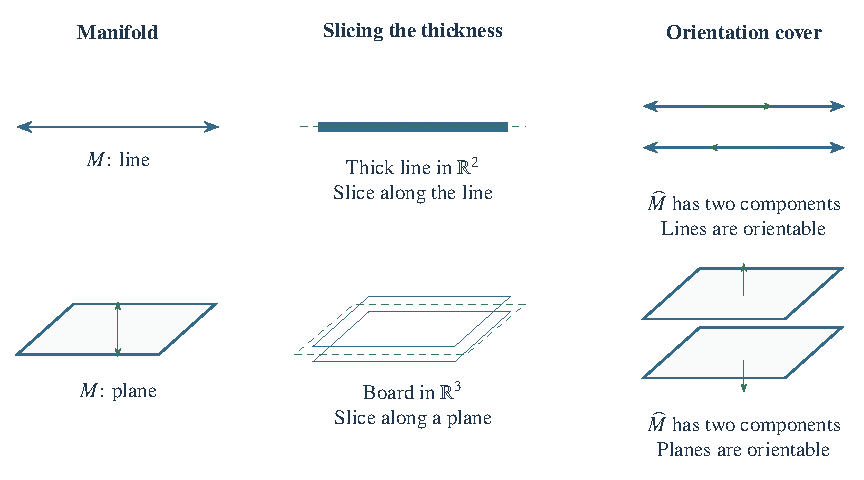
\includegraphics[width=.95\textwidth]{m4-fig-02.pdf}
 \FigureTag{M4.2}{fig:m4-fig-02}
\end{figure}
You will not obtain something similar if you slice a M\"obius band.
There, after slicing, the orientation cover $\widehat M$ remains connected.
Beyond offering this geometric insight into orientability, there are
mathematical reasons substantiating the Orientation Covering Theorem.
% Source page 9
\setcounter{theorem}{16}\begin{proposition}
Let $M$ be a connected smooth manifold. If $\pi_1(M)$ has no subgroup of
index $2$, then $M$ is orientable. In particular, all simply connected
smooth manifolds are orientable.
\end{proposition}
\begin{remark}
If $M$ were simply connected and covered something orientable, say
$\pi\colon M\to M/{\sim}$ with $M/{\sim}$ orientable, then $\pi$, being
a smooth covering map, is a local diffeomorphism. Hence $M$ is orientable.
\end{remark}
With this, we conclude.
% BLOG-CONTENT-END
\end{document}
